\documentclass[aspectratio=169,12pt]{beamer}

\usepackage[utf8]{inputenc}
\usepackage{amsmath,amssymb,bm}
\usepackage{booktabs}
\usepackage{ragged2e}
\usepackage{tikz}
\usetikzlibrary{arrows.meta,positioning,shapes.misc}

% ============================================================
% THEME — clean, large text, minimal clutter
% ============================================================
\usetheme{Madrid}
\usecolortheme{whale}
\setbeamertemplate{navigation symbols}{}
\setbeamertemplate{footline}[frame number]

\setbeamersize{
    text margin left=0.5cm,
    text margin right=0.5cm
}
\setbeamertemplate{frametitle}{%
  \nointerlineskip%
  \begin{beamercolorbox}[wd=\paperwidth,ht=2.8ex,dp=1.2ex,leftskip=0.5cm,rightskip=0.5cm]{frametitle}%
    \insertframetitle
  \end{beamercolorbox}%
}

\setlength{\leftmargini}{1.2em}
\setlength{\itemsep}{0.3em}
\setlength{\parskip}{0.3em}

% ============================================================
\title[Swift -- Simplified View]
{Swift: Persistent Fault-Tolerant UAV-IoT Networks}
\subtitle{Concept Map \textrightarrow\ Mathematical Formulation}
\author{Team -- Intelligent UAV Deployment}
\institute{IIT Dharwad -- ML in Wireless Networks}
\date{}

\begin{document}

% ============================================================
% SLIDE 1 — Title
% ============================================================
\begin{frame}
    \titlepage
\end{frame}

% ============================================================
% SLIDE 2 — Roadmap
% ============================================================
\begin{frame}{How to Read This Talk}
\begin{center}
\large
\textbf{Part A} \textrightarrow\ Plain-language idea \\[0.5em]
\textbf{Part B} \textrightarrow\ Same idea in math
\end{center}

\vspace{0.5em}
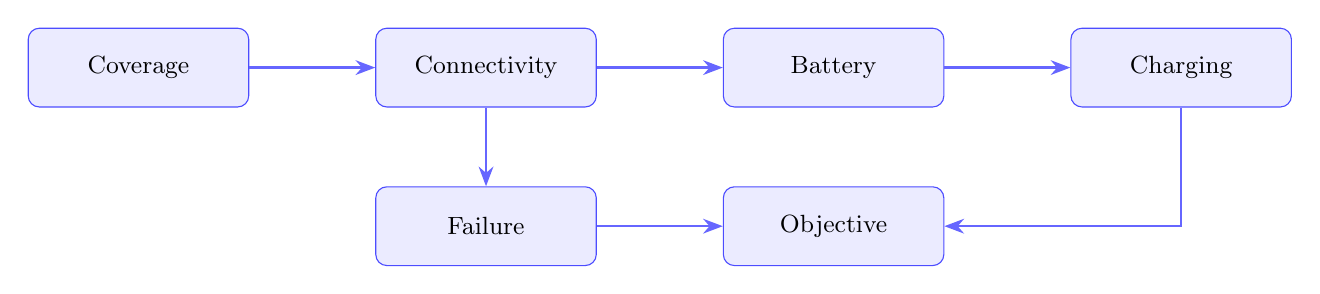
\begin{tikzpicture}[
    node distance=1.6cm,
    box/.style={rectangle, draw=blue!70, fill=blue!8, rounded corners,
                minimum height=1cm, minimum width=2.8cm, align=center, font=\small},
    arr/.style={-{Stealth[length=2.5mm]}, thick, blue!60}
]
\node[box] (a) {Coverage};
\node[box, right=of a] (b) {Connectivity};
\node[box, right=of b] (c) {Battery};
\node[box, right=of c] (d) {Charging};
\node[box, below=1.0cm of b] (e) {Failure};
\node[box, right=of e] (f) {Objective};
\draw[arr] (a) -- (b);
\draw[arr] (b) -- (c);
\draw[arr] (c) -- (d);
\draw[arr] (b) -- (e);
\draw[arr] (e) -- (f);
\draw[arr] (d) |- (f);
\end{tikzpicture}

\vspace{0.5em}
Each pair of slides: \textbf{idea} first, \textbf{equation} second.
\end{frame}

% ============================================================
% ============================================================
%  PART 1: THE PROBLEM
% ============================================================
% ============================================================

% --- SLIDE 3: Concept ---
\begin{frame}{The Problem (Idea)}
\begin{center}
\large
\textbf{We have} $N$ \textbf{drones} flying over $M$ \textbf{ground sensors}.\\[0.6em]
\end{center}

\vspace{0.3em}
Each drone has a battery that drains. Drones can \textbf{die}.\\
Sensors need \textbf{continuous coverage} --- at least $K$ drones above each.

\vspace{0.5em}
\begin{center}
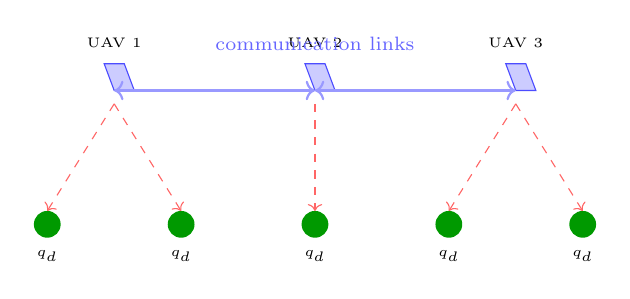
\begin{tikzpicture}[scale=0.85]
  % ground targets
  \foreach \x in {1,3,5,7,9} {
    \fill[green!60!black] (\x,0) circle(0.2);
    \node[below, font=\tiny] at (\x,-0.25) {$q_{d}$};
  }
  % UAVs
  \foreach \x/\lab in {2/1,5/2,8/3} {
    \filldraw[fill=blue!20, draw=blue!70] (\x,2) -- ++(0.3,0) -- ++(-0.15,0.4) -- ++(-0.3,0) -- cycle;
    \node[above, font=\tiny] at (\x,2.5) {UAV \lab};
  }
  % coverage arrows
  \draw[->,dashed,red!60] (2,1.8) -- (1,0.2);
  \draw[->,dashed,red!60] (2,1.8) -- (3,0.2);
  \draw[->,dashed,red!60] (5,1.8) -- (5,0.2);
  \draw[->,dashed,red!60] (8,1.8) -- (7,0.2);
  \draw[->,dashed,red!60] (8,1.8) -- (9,0.2);
  % comm link
  \draw[<->,thick,blue!40] (2,2) -- (5,2);
  \draw[<->,thick,blue!40] (5,2) -- (8,2);
  \node[font=\scriptsize, blue!60] at (5,2.7) {communication links};
\end{tikzpicture}
\end{center}

\vspace{0.3em}
\textbf{Challenge:} coordinate the drones with \emph{no central controller} so coverage never drops.
\end{frame}

% --- SLIDE 4: Math ---
\begin{frame}{The Problem (Math)}
We model the swarm as a \textbf{Dec-POMDP}:
\[
\mathcal{G} = \bigl\langle\,
  \underbrace{N}_{\text{agents}},\;
  \underbrace{\mathcal{S}}_{\text{state}},\;
  \underbrace{\{\mathcal{A}_i\}}_{\text{actions}},\;
  \underbrace{\{\mathcal{O}_i\}}_{\text{observations}},\;
  \underbrace{\mathcal{T}}_{\text{dynamics}},\;
  \underbrace{R}_{\text{reward}},\;
  \underbrace{\gamma}_{\text{discount}}
\,\bigr\rangle
\]

\vspace{0.4em}
\textbf{Objective:} find a policy $\pi$ that maximises expected cumulative reward:
\[
\max_{\pi}\;
\mathbb{E}_{\pi}
\!\left[
  \sum_{t=0}^{T} \gamma^{t}\, R_t
\right]
\]

\vspace{0.4em}
\begin{block}{What each piece means}
\begin{tabular}{@{}ll@{}}
$N$ & number of active UAV agents \\
$\mathcal{S}$ & every possible system configuration \\
$\mathcal{A}_i$ & what UAV $i$ can do (move, hover, charge) \\
$\mathcal{O}_i$ & what UAV $i$ can see locally \\
$\mathcal{T}$ & how the world transitions \\
$R$ & cooperative reward signal \\
$\gamma \in [0,1)$ & how much we value the future \\
\end{tabular}
\end{block}
\end{frame}

% ============================================================
% ============================================================
%  PART 2: STATE  --  what the world looks like
% ============================================================
% ============================================================

% --- SLIDE 5: Concept ---
\begin{frame}{What Does the World Look Like? (Idea)}
Each second, the \textbf{entire system} has a snapshot:

\begin{enumerate}
    \item \textbf{Where every drone is} and how much charge it has left.
    \item \textbf{Where every ground sensor is} and whether it has enough drones above it.
    \item \textbf{Which charging pads are free} and whether any drone just died.
\end{enumerate}

\vspace{0.6em}
\begin{center}
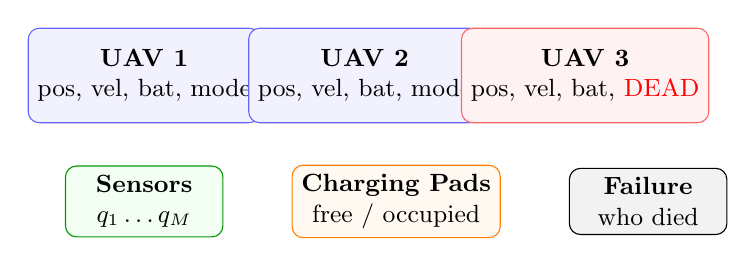
\begin{tikzpicture}[scale=0.8, every node/.style={font=\small}]
  % UAV info boxes
  \node[draw=blue!60, fill=blue!5, rounded corners, minimum width=2.5cm, minimum height=1.2cm, align=center] at (0,1.5) {\textbf{UAV 1}\\pos, vel, bat, mode};
  \node[draw=blue!60, fill=blue!5, rounded corners, minimum width=2.5cm, minimum height=1.2cm, align=center] at (3.5,1.5) {\textbf{UAV 2}\\pos, vel, bat, mode};
  \node[draw=red!60, fill=red!5, rounded corners, minimum width=2.5cm, minimum height=1.2cm, align=center] at (7,1.5) {\textbf{UAV 3}\\pos, vel, bat, \textcolor{red}{DEAD}};
  \node[draw=green!60!black, fill=green!5, rounded corners, minimum width=2cm, minimum height=0.8cm, align=center] at (0,-0.5) {\textbf{Sensors}\\$q_1\ldots q_M$};
  \node[draw=orange, fill=orange!5, rounded corners, minimum width=2cm, minimum height=0.8cm, align=center] at (4,-0.5) {\textbf{Charging Pads}\\free / occupied};
  \node[draw=black, fill=gray!10, rounded corners, minimum width=2cm, minimum height=0.8cm, align=center] at (8,-0.5) {\textbf{Failure}\\who died};
\end{tikzpicture}
\end{center}

This snapshot is the \textbf{state} $s_t$.
\end{frame}

% --- SLIDE 6: Math ---
\begin{frame}{State Definition (Math)}
\[
s_t = \Bigl\{
  \underbrace{(p_i,\; v_i,\; b_i,\; m_i)}_{\text{UAV $i$ info}},
  \;\;
  \underbrace{(q_d)_{d=1}^{M}}_{\text{sensor positions}},
  \;\;
  \underbrace{Q_t}_{\text{charging pads}},
  \;\;
  \underbrace{F_t}_{\text{failures}}
\Bigr\}
\]

\vspace{0.5em}
\begin{center}
\begin{tabular}{@{}lll@{}}
\toprule
\textbf{Symbol} & \textbf{Meaning} & \textbf{Range} \\
\midrule
$p_i$ & position of UAV $i$ & $(x,y,z) \in \mathbb{R}^3$ \\
$v_i$ & velocity of UAV $i$ & $\|v_i\| \le v_{\max}$ \\
$b_i$ & battery level & $[0, 1]$ (normalised) \\
$m_i$ & operating mode & \{serve, transit, charge\} \\
$q_d$ & position of sensor $d$ & fixed \\
$Q_t$ & charging pad occupancy & $\{0,1\}^S$ \\
$F_t$ & which UAVs failed & $\{0,1\}^N$ \\
\bottomrule
\end{tabular}
\end{center}

\vspace{0.4em}
\begin{block}{Key point}
During \textbf{training} the centralised critic sees all of $s_t$.
During \textbf{execution} each UAV only sees its own local observation (next slide).
\end{block}
\end{frame}

% ============================================================
% ============================================================
%  PART 3: LOCAL OBSERVATION  --  what each drone sees
% ============================================================
% ============================================================

% --- SLIDE 7: Concept ---
\begin{frame}{What Can Each Drone See? (Idea)}
A drone \textbf{cannot see everything}. It only knows:

\begin{itemize}
    \item Its \textbf{own} position, velocity, battery.
    \item Which \textbf{neighbour drones} are nearby (within radio range).
    \item How many sensors are covered \textbf{in its local area}.
    \item Whether it is a \textbf{single point of failure} for connectivity.
    \item \textbf{How far} the nearest charging station is.
\end{itemize}

\vspace{0.5em}
\begin{center}
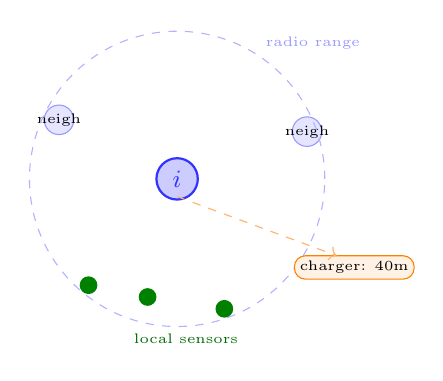
\begin{tikzpicture}[scale=0.75]
  % UAV i
  \filldraw[fill=blue!20, draw=blue!80, thick] (0,1) circle(0.35);
  \node[font=\small, blue!80] at (0,1) {$i$};
  % neighbours
  \filldraw[fill=blue!10, draw=blue!40] (-2,2) circle(0.25);
  \node[font=\tiny] at (-2,2) {neigh};
  \filldraw[fill=blue!10, draw=blue!40] (2.2,1.8) circle(0.25);
  \node[font=\tiny] at (2.2,1.8) {neigh};
  % comm range
  \draw[dashed, blue!30] (0,1) circle(2.5);
  \node[font=\tiny, blue!40] at (2.3,3.3) {radio range};
  % sensors nearby
  \fill[green!50!black] (-0.5,-1) circle(0.15);
  \fill[green!50!black] (0.8,-1.2) circle(0.15);
  \fill[green!50!black] (-1.5,-0.8) circle(0.15);
  \node[font=\tiny, green!40!black] at (0.15,-1.7) {local sensors};
  % charging station
  \node[draw=orange, fill=orange!10, rounded corners, font=\tiny, inner sep=2pt] at (3,-0.5) {charger: 40m};
  \draw[->, dashed, orange!60] (0,0.7) -- (2.7,-0.3);
\end{tikzpicture}
\end{center}

This partial view is the \textbf{local observation} $o_i$.
\end{frame}

% --- SLIDE 8: Math ---
\begin{frame}{Local Observation (Math)}
\[
o_i = \bigl[
  \underbrace{p_i,\; v_i,\; b_i}_{\text{own state}},\;\;
  \underbrace{\mathcal{N}_i}_{\text{neighbours}},\;\;
  \underbrace{C_i^{\text{local}}}_{\text{local coverage}},\;\;
  \underbrace{\text{risk}_i}_{\text{cut-vertex?}},\;\;
  \underbrace{t_i^{\text{empty}}}_{\text{time-to-empty}},\;\;
  \underbrace{E_i^{\text{station}}}_{\text{station energy}}
\bigr]
\]

\vspace{0.5em}
\begin{tabular}{@{}ll@{}}
\toprule
\textbf{Symbol} & \textbf{Meaning} \\
\midrule
$\mathcal{N}_i$ & indices of UAVs within $R_{\text{comm}}$ of UAV $i$ \\
$C_i^{\text{local}}$ & how many sensors near UAV $i$ are covered \\
$\text{risk}_i$ & $=1$ if removing UAV $i$ disconnects the swarm \\
$t_i^{\text{empty}}$ & seconds until battery hits the return threshold \\
$E_i^{\text{station}}$ & energy cost to reach the nearest pad \\
\bottomrule
\end{tabular}

\vspace{0.4em}
\begin{alertblock}{No central brain}
At execution time every UAV runs its own policy $\pi_\theta(a_i \mid o_i)$
using only $o_i$ --- no global state needed.
\end{alertblock}
\end{frame}

% ============================================================
% ============================================================
%  PART 4: WHY DECENTRALISED?
% ============================================================
% ============================================================

% --- SLIDE 9: Concept ---
\begin{frame}{Why Not One Central Controller? (Idea)}
With 1 central controller choosing actions for all $N$ drones:

\begin{center}
\large
\textbf{Action space grows exponentially} with the number of drones.
\end{center}

\vspace{0.5em}
\begin{center}
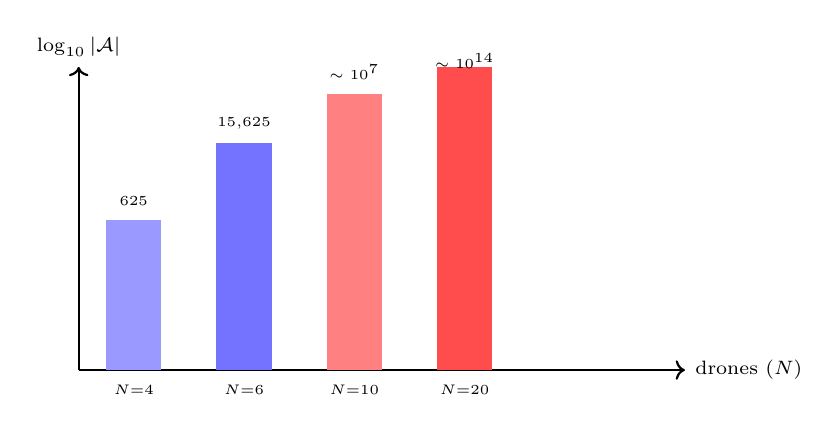
\begin{tikzpicture}[scale=0.7]
  % bar chart of action space
  \draw[->, thick] (0,0) -- (11,0) node[right, font=\scriptsize] {drones ($N$)};
  \draw[->, thick] (0,0) -- (0,5.5) node[above, font=\scriptsize] {$\log_{10}|\mathcal{A}|$};
  % bars
  \fill[blue!40] (0.5,0) rectangle (1.5,2.72);  % N=4, 625
  \node[below, font=\tiny] at (1,-0.1) {$N{=}4$};
  \node[above, font=\tiny] at (1,2.8) {$625$};
  \fill[blue!55] (2.5,0) rectangle (3.5,4.12);  % N=6
  \node[below, font=\tiny] at (3,-0.1) {$N{=}6$};
  \node[above, font=\tiny] at (3,4.2) {$15{,}625$};
  \fill[red!50] (4.5,0) rectangle (5.5,5.0);    % N=10
  \node[below, font=\tiny] at (5,-0.1) {$N{=}10$};
  \node[above, font=\tiny] at (5,5.1) {$\sim10^7$};
  \fill[red!70] (6.5,0) rectangle (7.5,5.5);    % N=20
  \node[below, font=\tiny] at (7,-0.1) {$N{=}20$};
  \node[above, font=\tiny] at (7,5.3) {$\sim10^{14}$};
\end{tikzpicture}
\end{center}

\vspace{0.3em}
\textbf{Solution:} let each drone decide \emph{for itself}, using only what it can see.
\end{frame}

% --- SLIDE 10: Math ---
\begin{frame}{Decentralised Policy (Math)}
\textbf{Centralised:}
$|\mathcal{A}| = A^N$ where $A = |\mathcal{A}_i|$

\vspace{0.3em}

\textbf{Factorised (ours):} each UAV picks its own action:
\[
a_i \sim \pi_\theta(a_i \mid o_i)
\qquad \Longrightarrow \qquad
|\mathcal{A}|_{\text{eff}} = A \;\text{(per agent)}
\]

\vspace{0.5em}
\begin{center}
\begin{tabular}{@{}ccccc@{}}
\toprule
$N$ & 4 & 6 & 10 & 20 \\
\midrule
Centralised & $5^4{=}625$ & $5^6{=}15{,}625$ & $\sim10^7$ & $\sim10^{14}$ \\
Decentralised & 5 & 5 & 5 & 5 \\
\bottomrule
\end{tabular}
\end{center}

\vspace{0.4em}
\begin{block}{Trade-off}
Decentralised is tractable, but individual drones have \emph{partial information}.
The observation $o_i$ must carry enough context for good coordination.
\end{block}
\end{frame}

% ============================================================
% ============================================================
%  PART 5: ACTION SPACE
% ============================================================
% ============================================================

% --- SLIDE 11: Concept ---
\begin{frame}{What Can a Drone Do? (Idea)}
Each drone picks \textbf{one action per time step}:

\begin{center}
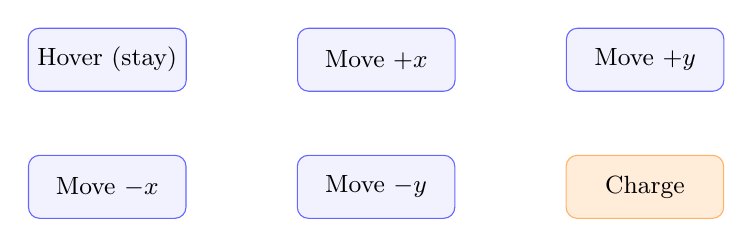
\begin{tikzpicture}[
    node distance=0.8cm and 1.4cm,
    act/.style={rectangle, draw=blue!60, fill=blue!5, rounded corners,
                minimum height=0.8cm, minimum width=2.0cm, align=center, font=\small},
    arr/.style={-{Stealth[length=2mm]}, blue!50}
]
\node[act] (h) {Hover (stay)};
\node[act, right=of h] (ux) {Move $+x$};
\node[act, right=of ux] (uy) {Move $+y$};
\node[act, below=of h] (dx) {Move $-x$};
\node[act, right=of dx] (dy) {Move $-y$};
\node[act, right=of dy, fill=orange!15, draw=orange!60] (ch) {Charge};
\end{tikzpicture}
\end{center}

\vspace{0.4em}
\textbf{Hover:} stay in place, keep covering sensors.\\
\textbf{Move:} fly one step in a cardinal direction.\\
\textbf{Charge:} if at a pad, recharge battery.
\end{frame}

% --- SLIDE 12: Math ---
\begin{frame}{Action Space (Math)}
\[
\mathcal{A}_i = \bigl\{
  \text{Hover},\;
  {+x},\; {-x},\; {+y},\; {-y},\;
  \text{Charge}
\bigr\}, \quad |\mathcal{A}_i| = 6
\]

\vspace{0.4em}
\textbf{Movement constraint:}
\[
p_i(t+1) = p_i(t) + v_i(t) \cdot \Delta t,
\qquad \|v_i(t)\| \le v_{\max}, \quad p_i \in \Omega
\]
where $\Omega$ is the airspace boundary.

\vspace{0.4em}
\textbf{Charge action is only valid when:}
\[
\|p_i - p_s^{\text{pad}}\| \le d_{\text{charge}},
\quad Q_t[s] = 1 \;\text{(pad is free)}
\]
Otherwise the action defaults to \emph{Hover}.
\end{frame}

% ============================================================
% ============================================================
%  PART 6: K-COVERAGE
% ============================================================
% ============================================================

% --- SLIDE 13: Concept ---
\begin{frame}{K-Coverage (Idea)}
\begin{block}{Rule}
Every ground sensor must have \textbf{at least $K$ drones} above it at all times.
\end{block}

\vspace{0.3em}
\begin{center}
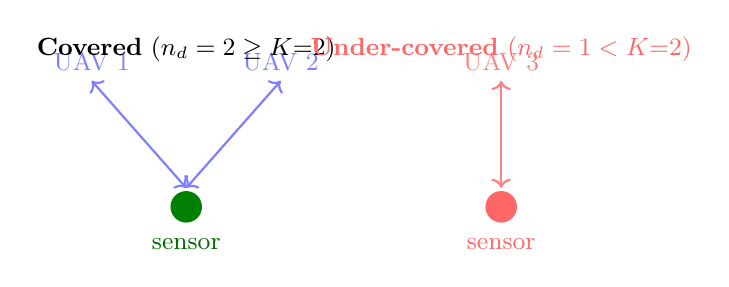
\begin{tikzpicture}[scale=0.8]
  % sensor
  \fill[green!50!black] (0,0) circle(0.25);
  \node[below, font=\small, green!40!black] at (0,-0.35) {sensor};
  % K=2 coverage
  \draw[<->, thick, blue!50] (-1.5,2) node[above, font=\small]{UAV 1} -- (0,0.3);
  \draw[<->, thick, blue!50] (1.5,2) node[above, font=\small]{UAV 2} -- (0,0.3);
  \node[font=\small] at (0,2.5) {\textbf{Covered} ($n_d = 2 \ge K{=}2$)};
  % uncovered
  \fill[red!60] (5,0) circle(0.25);
  \node[below, font=\small, red!60] at (5,-0.35) {sensor};
  \draw[<->, thick, red!50] (5,2) node[above, font=\small]{UAV 3} -- (5,0.3);
  \node[font=\small, red!60] at (5,2.5) {\textbf{Under-covered} ($n_d = 1 < K{=}2$)};
\end{tikzpicture}
\end{center}

\vspace{0.3em}
We want \textbf{zero under-covered sensors} for as much of the mission as possible.
\end{frame}

% --- SLIDE 14: Math ---
\begin{frame}{K-Coverage (Math)}
\textbf{Binary coverage} --- is UAV $i$ covering sensor $d$?
\[
x_{id}(t) = \mathbf{1}\!\bigl[\,\|p_i(t) - q_d\| \le R_{\text{cov}}\,\bigr]
\]

\vspace{0.3em}
\textbf{Coverage count} for sensor $d$:
\[
n_d(t) = \sum_{i=1}^{N} x_{id}(t)
\]

\vspace{0.3em}
\textbf{Coverage score} (fraction of sensors adequately covered):
\[
C(t) = \frac{1}{M}\sum_{d=1}^{M} \min\!\left(\frac{n_d(t)}{K},\; 1\right)
\]

\vspace{0.3em}
\textbf{Under-coverage rate} (what we want to minimise):
\[
U(t) = \frac{1}{M}\sum_{d=1}^{M} \mathbf{1}\!\bigl[\,n_d(t) < K\,\bigr]
\]
\end{frame}

% ============================================================
% ============================================================
%  PART 7: CONNECTIVITY
% ============================================================
% ============================================================

% --- SLIDE 15: Concept ---
\begin{frame}{Connectivity (Idea)}
Drones must \textbf{talk to each other} to coordinate.\\
Two drones can communicate if they are within radio range $R_{\text{comm}}$.

\vspace{0.4em}
\begin{center}
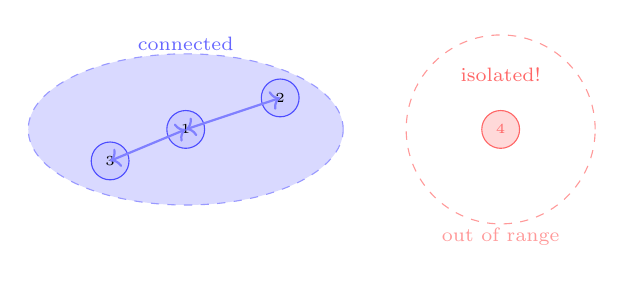
\begin{tikzpicture}[scale=0.8]
  % connected component
  \filldraw[fill=blue!15, draw=blue!40, dashed] (0,1) ellipse(2.5cm and 1.2cm);
  \node[above, font=\scriptsize, blue!60] at (0,2.1) {connected};
  \filldraw[fill=blue!20, draw=blue!70] (0,1) circle(0.3);
  \node[font=\tiny] at (0,1) {$1$};
  \filldraw[fill=blue!20, draw=blue!70] (1.5,1.5) circle(0.3);
  \node[font=\tiny] at (1.5,1.5) {$2$};
  \filldraw[fill=blue!20, draw=blue!70] (-1.2,0.5) circle(0.3);
  \node[font=\tiny] at (-1.2,0.5) {$3$};
  \draw[<->, thick, blue!50] (0,1) -- (1.5,1.5);
  \draw[<->, thick, blue!50] (0,1) -- (-1.2,0.5);
  % isolated drone
  \filldraw[fill=red!15, draw=red!60] (5,1) circle(0.3);
  \node[font=\tiny, red!60] at (5,1) {$4$};
  \node[above, font=\scriptsize, red!60] at (5,1.6) {isolated!};
  \draw[red!40, dashed] (5,1) circle(1.5);
  \node[font=\scriptsize, red!40] at (5,-0.7) {out of range};
\end{tikzpicture}
\end{center}

\vspace{0.3em}
If removing one drone \textbf{splits} the group, that drone is a \textbf{cut-vertex} --- high risk.
\end{frame}

% --- SLIDE 16: Math ---
\begin{frame}{Connectivity (Math)}
\textbf{Communication graph:}
\[
G_t = (V, E_t),
\quad
E_t = \bigl\{(i,j) : \|p_i - p_j\| \le R_{\text{comm}}\bigr\}
\]

\vspace{0.4em}
\textbf{Connectivity risk} --- is UAV $i$ a cut-vertex?
\[
\text{risk}_i(t) = \mathbf{1}\!\bigl[\,G_t^{-i} \text{ is disconnected}\,\bigr]
\]
where $G_t^{-i}$ is the graph with UAV $i$ and its edges removed.

\vspace{0.4em}
\begin{block}{Why this matters}
A drone that is the \emph{only link} between two parts of the swarm
should \textbf{not} leave for charging without a replacement taking its place.
\end{block}

\vspace{0.3em}
\textbf{Desired global property:}
\[
G_t \text{ is connected} \quad \forall\, t
\]
\end{frame}

% ============================================================
% ============================================================
%  PART 8: BATTERY MODEL
% ============================================================
% ============================================================

% --- SLIDE 17: Concept ---
\begin{frame}{Battery Model (Idea)}
Every drone burns energy doing three things:

\begin{enumerate}
    \item \textbf{Hovering} --- staying airborne.
    \item \textbf{Moving} --- flying to a new position.
    \item \textbf{Communicating} --- sending data to neighbours.
\end{enumerate}

\vspace{0.4em}
\begin{center}
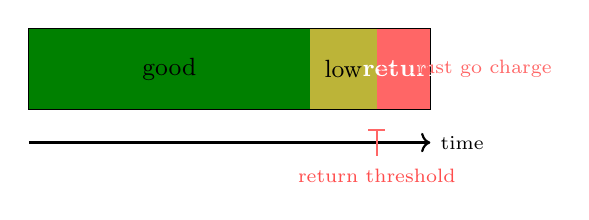
\begin{tikzpicture}[scale=0.85]
  % battery
  \draw[thick] (0,0) rectangle (6,1.2);
  \fill[green!50!black] (0,0) rectangle (4.2,1.2);
  \fill[yellow!70!black] (4.2,0) rectangle (5.2,1.2);
  \fill[red!60] (5.2,0) rectangle (6,1.2);
  \node[font=\small] at (2.1,0.6) {good};
  \node[font=\small] at (4.7,0.6) {low};
  \node[font=\small, white] at (5.6,0.6) {\textbf{return}};
  \node[font=\scriptsize, red!60] at (6.5,0.6) {$\leftarrow$ must go charge};
  % arrows
  \draw[->, thick] (0,-0.5) -- (6,-0.5) node[right, font=\scriptsize] {time};
  \node[font=\scriptsize, red!70] at (5.2,-1) {return threshold};
  \draw[|-, red!60, thick] (5.2,-0.3) -- (5.2,-0.7);
\end{tikzpicture}
\end{center}

When battery hits the \textbf{return threshold}, the drone \emph{must} go charge.
\end{frame}

% --- SLIDE 18: Math ---
\begin{frame}{Battery Model (Math)}
\[
b_i(t+\Delta t) = b_i(t)
+ \underbrace{\frac{-P_{\text{hover}} - P_{\text{move}} - P_{\text{comm}}}{B_i^{\max}}\,\Delta t}_{\text{drain}}
+ \underbrace{\Delta b_i^{\text{charge}}}_{\text{recharge (at pad)}}
\]

\vspace{0.4em}
\textbf{Return-to-charge condition:}
\[
b_i(t) \cdot B_i^{\max}
\;\le\;
E_i^{\text{req}}
= E_i^{\text{station}} + E_i^{\text{return}} + E^{\text{reserve}}
\]

\vspace{0.3em}
\begin{tabular}{@{}ll@{}}
\toprule
\textbf{Symbol} & \textbf{Meaning} \\
\midrule
$b_i(t)$ & normalised battery $[0,1]$ \\
$P_{\text{hover}}$ & power consumed hovering (W) \\
$P_{\text{move}}$ & power consumed moving (W) \\
$P_{\text{comm}}$ & power consumed communicating (W) \\
$B_i^{\max}$ & total battery capacity (J) \\
$E_i^{\text{station}}$ & energy to reach nearest pad \\
$E_i^{\text{return}}$ & energy to return from pad to current area \\
$E^{\text{reserve}}$ & safety margin \\
\bottomrule
\end{tabular}
\end{frame}

% ============================================================
% ============================================================
%  PART 9: CHARGING COORDINATION
% ============================================================
% ============================================================

% --- SLIDE 19: Concept ---
\begin{frame}{Charging Coordination (Idea)}
Multiple drones may need to charge simultaneously, but pads are limited.

\vspace{0.4em}
\begin{center}
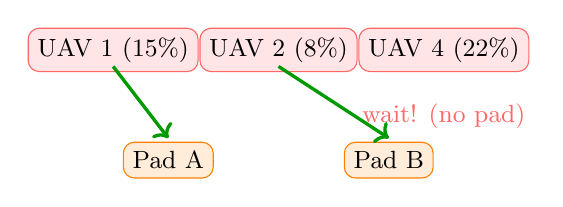
\begin{tikzpicture}[scale=0.7]
  % drones needing charge
  \node[draw=red!60, fill=red!10, rounded corners, font=\small] at (0,2) {UAV 1 (15\%)};
  \node[draw=red!60, fill=red!10, rounded corners, font=\small] at (3,2) {UAV 2 (8\%)};
  \node[draw=red!60, fill=red!10, rounded corners, font=\small] at (6,2) {UAV 4 (22\%)};
  % pads
  \node[draw=orange, fill=orange!15, rounded corners, font=\small] at (1,0) {Pad A};
  \node[draw=orange, fill=orange!15, rounded corners, font=\small] at (5,0) {Pad B};
  % assignment arrows
  \draw[->, very thick, green!60!black] (0,1.7) -- (1,0.4);
  \draw[->, very thick, green!60!black] (3,1.7) -- (5,0.4);
  \node[font=\small, red!60, align=center] at (6,0.8) {wait! (no pad)};
\end{tikzpicture}
\end{center}

\vspace{0.3em}
We solve a \textbf{min-cost assignment} every time a drone requests a pad.
\end{frame}

% --- SLIDE 20: Math ---
\begin{frame}{Charging Coordination (Math)}
\textbf{Decision variable:}
$y_{is} \in \{0,1\}$ \textbf{---} assign UAV $i$ to pad $s$?

\vspace{0.3em}
\textbf{Cost:}
\[
c_{is} = \alpha\, d_{is} + \beta\, q_s + \mu\, u_i
\]
where $d_{is}$ = distance, $q_s$ = queue length at pad, $u_i$ = urgency.

\vspace{0.3em}
\textbf{Optimisation:}
\[
\min_{y}\; \sum_{i}\sum_{s}\; c_{is}\, y_{is}
\]

\vspace{0.3em}
\textbf{Constraints:}
\[
\sum_{s} y_{is} \le 1 \;\;\forall\, i
\qquad\text{(each UAV $\le$ 1 pad)},
\qquad
\sum_{i} y_{is} \le 1 \;\;\forall\, s
\qquad\text{(each pad $\le$ 1 UAV)}
\]

\vspace{0.3em}
\begin{tabular}{@{}ll@{}}
\toprule
\textbf{Symbol} & \textbf{Meaning} \\
\midrule
$\alpha$ & weight for distance to station \\
$\beta$ & weight for station queue length \\
$\mu$ & weight for urgency (battery depletion risk) \\
\bottomrule
\end{tabular}

\vspace{0.3em}
For pairwise assignment, the \textbf{Hungarian algorithm} solves this efficiently.
\end{frame}

% ============================================================
% ============================================================
%  PART 10: OBJECTIVE FUNCTION
% ============================================================
% ============================================================

% --- SLIDE 21: Concept ---
\begin{frame}{The Goal (Idea)}
We are balancing \textbf{6 competing objectives}:

\vspace{0.3em}
\begin{center}
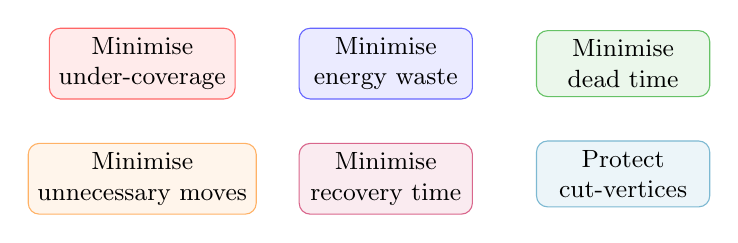
\begin{tikzpicture}[
    node distance=0.55cm and 0.8cm,
    obj/.style={rectangle, draw=#1!60, fill=#1!8, rounded corners,
                minimum height=0.65cm, minimum width=2.2cm, align=center, font=\small}
]
\node[obj=red] (U) {Minimise\\under-coverage};
\node[obj=blue, right=of U] (E) {Minimise\\energy waste};
\node[obj=green!60!black, right=of E] (D) {Minimise\\dead time};
\node[obj=orange, below=of U] (W) {Minimise\\unnecessary moves};
\node[obj=purple, below=of E] (R) {Minimise\\recovery time};
\node[obj=cyan!70!black, below=of D] (C) {Protect\\cut-vertices};
\end{tikzpicture}
\end{center}

\vspace{0.4em}
Each objective gets a \textbf{weight} $\lambda$ to control importance.
\end{frame}

% --- SLIDE 22: Math ---
\begin{frame}{Multi-Objective Formulation (Math)}
\[
\min_{\pi}\;
\mathbb{E}_{\pi}
\!\left[
\sum_{t=0}^{T-1}
\Bigl(
  \underbrace{\lambda_O\, U(t)}_{\text{under-coverage}}
  + \underbrace{\lambda_E\, E(t)}_{\text{energy waste}}
  + \underbrace{\lambda_D\, D(t)}_{\text{dead time}}
  + \underbrace{\lambda_W\, W(t)}_{\text{wasted moves}}
  + \underbrace{\lambda_R\, R(t)}_{\text{recovery}}
  + \underbrace{\lambda_C\, \text{Crit}(t)}_{\text{cut-vertex risk}}
\Bigr)
\right]
\]

\vspace{0.4em}
\begin{tabular}{@{}lll@{}}
\toprule
\textbf{Term} & \textbf{Definition} & \textbf{What it penalises} \\
\midrule
$U(t)$ & $\frac{1}{M}\sum_d \mathbf{1}[n_d{<}K]$ & sensors below $K$-coverage \\
$E(t)$ & fraction of flights with low battery & excessive energy drain \\
$D(t)$ & fraction of time in degraded state & time after a failure \\
$W(t)$ & moves that don't improve coverage & wasteful repositioning \\
$R(t)$ & $\min(t_{\text{recovered}}, t_{\text{cap}})$ & time to restore coverage \\
$\text{Crit}(t)$ & fraction of cut-vertices active & connectivity fragility \\
\bottomrule
\end{tabular}
\end{frame}

% ============================================================
% ============================================================
%  PART 11: CONSTRAINTS
% ============================================================
% ============================================================

% --- SLIDE 23: Concept ---
\begin{frame}{Safety Constraints (Idea)}
Drones must follow hard rules at \emph{every} time step:

\begin{enumerate}
    \item \textbf{Speed limit} --- don't fly too fast.
    \item \textbf{Stay inside} the designated airspace.
    \item \textbf{Don't collide} --- maintain safe distance from other drones.
\end{enumerate}

\vspace{0.5em}
\begin{center}
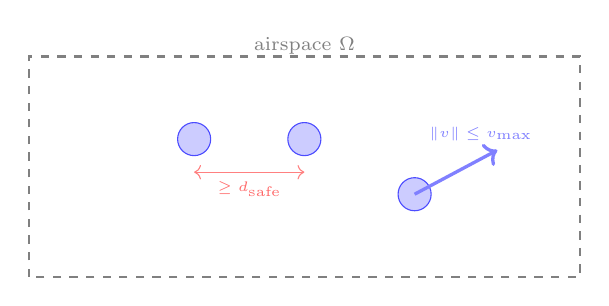
\begin{tikzpicture}[scale=0.7]
  % airspace boundary
  \draw[thick, dashed, gray] (-1,-0.5) rectangle (9,3.5);
  \node[font=\scriptsize, gray] at (4,3.7) {airspace $\Omega$};
  % drones
  \filldraw[fill=blue!20, draw=blue!70] (2,2) circle(0.3);
  \filldraw[fill=blue!20, draw=blue!70] (4,2) circle(0.3);
  \filldraw[fill=blue!20, draw=blue!70] (6,1) circle(0.3);
  % safe distance
  \draw[<->, red!50] (2,1.4) -- (4,1.4) node[midway, below, font=\tiny, red!60] {$\ge d_{\text{safe}}$};
  % velocity arrow
  \draw[->, very thick, blue!50] (6,1) -- (7.5,1.8);
  \node[font=\tiny, blue!50] at (7.2,2.1) {$\|v\| \le v_{\max}$};
\end{tikzpicture}
\end{center}
\end{frame}

% --- SLIDE 24: Math ---
\begin{frame}{Safety Constraints (Math)}
At every time step $t$, for all UAVs $i$:

\vspace{0.3em}
\begin{enumerate}
    \item \textbf{Speed:}
    $\|v_i(t)\| \le v_{\max}$
    \item \textbf{Workspace:}
    $p_i(t) \in \Omega \subset \mathbb{R}^3$
    \item \textbf{Collision avoidance:}
    $\|p_i(t) - p_j(t)\| \ge d_{\text{safe}}
    \quad \forall\, j \ne i$
\end{enumerate}

\vspace{0.6em}
\begin{block}{Hard vs soft}
These are \textbf{hard constraints} --- violated states are either
prevented (action masking) or heavily penalised in the reward.
\end{block}
\end{frame}

% ============================================================
% ============================================================
%  PART 12: FAILURE & RECOVERY
% ============================================================
% ============================================================

% --- SLIDE 25: Concept ---
\begin{frame}{What Happens When a Drone Dies? (Idea)}

\begin{center}
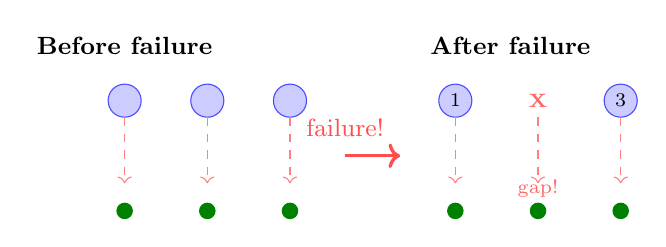
\begin{tikzpicture}[scale=0.7]
  % before failure
  \node[font=\small] at (0,3) {\textbf{Before failure}};
  \filldraw[fill=blue!20, draw=blue!70] (0,2) circle(0.3);
  \filldraw[fill=blue!20, draw=blue!70] (1.5,2) circle(0.3);
  \filldraw[fill=blue!20, draw=blue!70] (3,2) circle(0.3);
  \draw[->, dashed, red!50] (0,1.7) -- (0,0.5);
  \draw[->, dashed, red!50] (1.5,1.7) -- (1.5,0.5);
  \draw[->, dashed, red!50] (3,1.7) -- (3,0.5);
  \fill[green!50!black] (0,0) circle(0.15);
  \fill[green!50!black] (1.5,0) circle(0.15);
  \fill[green!50!black] (3,0) circle(0.15);
  % failure arrow
  \draw[->, very thick, red!70] (4,1) -- (5,1);
  \node[font=\small, red!70] at (4,1.5) {failure!};
  % after failure
  \node[font=\small] at (7,3) {\textbf{After failure}};
  \filldraw[fill=blue!20, draw=blue!70] (6,2) circle(0.3);
  \node[font=\scriptsize] at (6,2) {$1$};
  \filldraw[fill=blue!20, draw=blue!70] (9,2) circle(0.3);
  \node[font=\scriptsize] at (9,2) {$3$};
  \node[font=\scriptsize, red!60] at (7.5,2) {\textbf{X}};
  \draw[->, dashed, red!50] (6,1.7) -- (6,0.5);
  \draw[->, dashed, red!50] (9,1.7) -- (9,0.5);
  \draw[->, dashed, red!50] (7.5,1.7) -- (7.5,0.5);
  \fill[green!50!black] (6,0) circle(0.15);
  \fill[green!50!black] (7.5,0) circle(0.15);
  \fill[green!50!black] (9,0) circle(0.15);
  \node[font=\scriptsize, red!60] at (7.5,0.4) {gap!};
\end{tikzpicture}
\end{center}

We measure \textbf{how quickly} the remaining drones close the gap.
\end{frame}

% --- SLIDE 26: Math ---
\begin{frame}{Failure \& Recovery (Math)}
\textbf{Recovery time:} how long until coverage is restored after a failure at $t_f$:
\[
\tau_f = \inf\!\bigl\{\tau \ge 0 :
  n_d(t_f + \tau) \ge K \;\;\forall\, d \in \mathcal{M}\bigr\}
\]

\vspace{0.4em}
\textbf{Requirement:}
\[
\tau_f \le \tau_{\max}
\]

\vspace{0.4em}
\begin{block}{Reserve UAV strategy}
Keep 1 drone in reserve with $b_i > b_{\text{threshold}}$.\\
When a drone fails, the reserve immediately repositions to fill the gap, reducing $\tau_f$.
\end{block}

\vspace{0.3em}
\textbf{Reserve activation condition:}
\[
\text{reserve takes off when } F_t \text{ changes (new failure detected)}
\]
\end{frame}

% ============================================================
% ============================================================
%  PART 13: HOW THE AI LEARNS (MAPPO)
% ============================================================
% ============================================================

% --- SLIDE 27: Concept ---
\begin{frame}{How the AI Learns (Idea)}
We use \textbf{MAPPO} --- Multi-Agent Proximal Policy Optimisation.

\vspace{0.3em}
\begin{center}
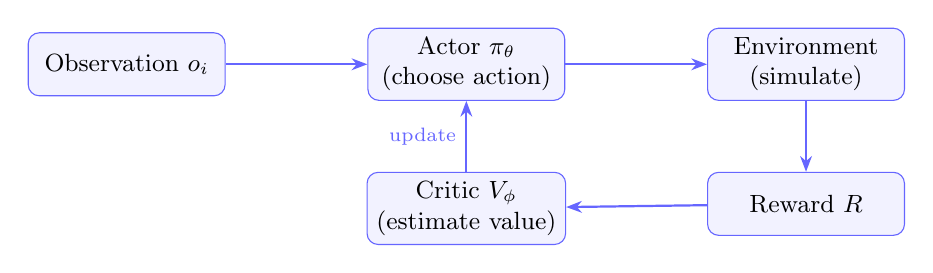
\begin{tikzpicture}[
    node distance=0.9cm,
    box/.style={rectangle, draw=blue!60, fill=blue!5, rounded corners,
                minimum height=0.8cm, minimum width=2.5cm, align=center, font=\small},
    arr/.style={-{Stealth[length=2mm]}, thick, blue!60}
]
\node[box] (obs) {Observation $o_i$};
\node[box, right=1.8cm of obs] (actor) {Actor $\pi_\theta$\\(choose action)};
\node[box, right=1.8cm of actor] (env) {Environment\\(simulate)};
\node[box, below=0.9cm of actor] (critic) {Critic $V_\phi$\\(estimate value)};
\node[box, below=0.9cm of env] (rew) {Reward $R$};
\draw[arr] (obs) -- (actor);
\draw[arr] (actor) -- (env);
\draw[arr] (env) -- (rew);
\draw[arr] (rew) -- (critic);
\draw[arr] (critic) -- (actor) node[midway, left, font=\scriptsize] {update};
\end{tikzpicture}
\end{center}

\vspace{0.3em}
\textbf{Centralised training, decentralised execution:} during training the critic sees all of $s_t$; at deployment each drone acts on $o_i$ alone.
\end{frame}

% --- SLIDE 28: Math ---
\begin{frame}{MAPPO (Math)}
\textbf{Actor} (per UAV): $a_i \sim \pi_\theta(a_i \mid o_i)$

\vspace{0.3em}
\textbf{Critic} (centralised, training only): $V_\phi(s_t)$

\vspace{0.3em}
\textbf{Actor loss} (PPO clipped):
\[
\mathcal{L}^{\text{actor}}(\theta)
= -\mathbb{E}_t\!\left[
  \min\!\left(
    r_t(\theta)\,\hat{A}_t,\;
    \text{clip}\bigl(r_t(\theta), 1{-}\epsilon, 1{+}\epsilon\bigr)\,\hat{A}_t
  \right)
\right]
\]
where $r_t(\theta) = \frac{\pi_\theta(a_t \mid o_t)}{\pi_{\theta_{\text{old}}}(a_t \mid o_t)}$ and $\hat{A}_t = R_t - V_\phi(s_t)$ (GAE advantage).

\vspace{0.3em}
\textbf{Critic loss:}
\[
\mathcal{L}^{\text{critic}}(\phi)
= \mathbb{E}_t\!\left[
  \bigl(R_t - V_\phi(s_t)\bigr)^2
\right]
\]

\vspace{0.3em}
\begin{tabular}{@{}ll@{}}
\toprule
\textbf{Hyperparameter} & \textbf{Value} \\
\midrule
Number of UAVs $N$ & 5 \\
IoT devices $M$ & 20 \\
Discount $\gamma$ & 0.99 \\
PPO clip $\epsilon$ & 0.2 \\
\bottomrule
\end{tabular}
\end{frame}

% ============================================================
% ============================================================
%  PART 14: IMPLEMENTATION SUMMARY
% ============================================================
% ============================================================

% --- SLIDE 29: Concept ---
\begin{frame}{Putting It All Together (Idea)}
\begin{center}
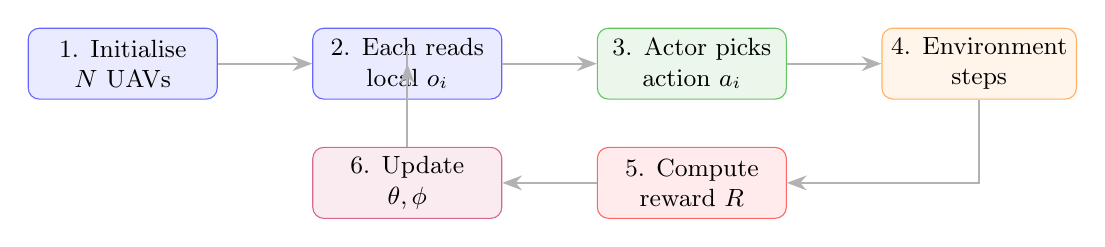
\begin{tikzpicture}[
    node distance=0.6cm and 1.2cm,
    step/.style={rectangle, draw=#1!60, fill=#1!8, rounded corners,
                 minimum height=0.9cm, minimum width=2.4cm, align=center, font=\small},
    arr/.style={-{Stealth[length=2.5mm]}, thick, gray!60}
]
\node[step=blue] (s1) {1. Initialise\\$N$ UAVs};
\node[step=blue, right=of s1] (s2) {2. Each reads\\local $o_i$};
\node[step=green!60!black, right=of s2] (s3) {3. Actor picks\\action $a_i$};
\node[step=orange, right=of s3] (s4) {4. Environment\\steps};
\node[step=red, below=of s3] (s5) {5. Compute\\reward $R$};
\node[step=purple, left=of s5] (s6) {6. Update\\$\theta, \phi$};
\draw[arr] (s1) -- (s2);
\draw[arr] (s2) -- (s3);
\draw[arr] (s3) -- (s4);
\draw[arr] (s4) |- (s5);
\draw[arr] (s5) -- (s6);
\draw[arr] (s6) |- (s2);
\end{tikzpicture}
\end{center}
\end{frame}

% --- SLIDE 30: Summary Table ---
\begin{frame}{Implementation Summary (Math + Values)}
\begin{center}
\small
\begin{tabular}{@{}lll@{}}
\toprule
\textbf{Component} & \textbf{Math} & \textbf{Value} \\
\midrule
Airspace & $\Omega$ & $100 \times 100 \times 30$ m$^3$ \\
UAVs & $N$ & 5 (+ 1 reserve) \\
Sensors & $M$ & 20 \\
Coverage radius & $R_{\text{cov}}$ & 15 m \\
Comm radius & $R_{\text{comm}}$ & 40 m \\
Min $K$-coverage & $K$ & 2 \\
Sim step & $\Delta t$ & 1 s \\
Max velocity & $v_{\max}$ & 5 m/s \\
Safe distance & $d_{\text{safe}}$ & 5 m \\
Battery capacity & $B^{\max}$ & 30\,000 J \\
Hover power & $P_{\text{hover}}$ & 50 W \\
Move power & $P_{\text{move}}$ & 75 W \\
Comm power & $P_{\text{comm}}$ & 10 W \\
Charge rate & $\Delta b^{\text{charge}}$ & 0.01/step \\
Discount & $\gamma$ & 0.99 \\
PPO clip & $\epsilon$ & 0.2 \\
\bottomrule
\end{tabular}
\end{center}
\end{frame}

% ============================================================
% SLIDE 31 — End
% ============================================================
\begin{frame}
\begin{center}
\vspace{1.5em}
\Large\textbf{Questions?}
\end{center}
\end{frame}

\end{document}
